\documentclass[11pt,oneside]{article} % typ dokumentu
\usepackage[utf8]{inputenc} % kódování

\usepackage{amsmath} % rovnice
\usepackage{amssymb} % další symboly
\usepackage{graphicx} % vkládání obrázků
\usepackage[czech]{babel} % formátování závislé na jazyku
\usepackage{fancyhdr} % Záhlaví a zápatí stránek
\usepackage{lastpage} % Odkaz na poslední stránku v zápatí
\usepackage{siunitx} % SI jednotky

% Geometrie stránky (okraje...)
\usepackage{geometry}
\geometry{
   a4paper,
   left=30mm,
   right=30mm,
   top=20mm,
   bottom=20mm,
   headheight=14pt,
   includeheadfoot
}

% Formátování textu v odstavci
\setlength{\parindent}{0pt}
\setlength{\parskip}{1.5em}
\renewcommand{\baselinestretch}{1.2}

% Nastavení záhlaví a zápatí
\fancypagestyle{titulni}
{
   \setlength{\headheight}{20mm}
   \fancyhf{} % Ruší globální nastavení
   \renewcommand{\headrulewidth}{0pt}
   \fancyhead[R]{\includegraphics[height=18mm]{obrazky/Logo_CVUT.pdf}}
   \fancyhead[L]{
      FAKULTA STROJNÍ \\
      ÚSTAV PŘÍSTROJOVÉ A ŘÍDÍCÍ TECHNIKY \\
      Automatické řízení (2371047)
   }
}

\pagestyle{fancy}
\renewcommand{\headrulewidth}{.5pt}
\fancyfoot[C]{Strana \thepage \ z \pageref{LastPage}}
\fancyhead[L]{\protokol}
\fancyhead[R]{\uloha}

% Bibliografické informace
\title{\protokol \\ \large \uloha}
\author{Honza Novák \and Jozef Kovář}
\def \uloha{FXX - název úlohy}
\def \protokol{Protokol z laboratorního cvičení}

\begin{document}

\maketitle
\thispagestyle{titulni}

\newpage

\section*{Zadání}

Laboratorní úlohou bylo vypočítat přítažnou sílu mezi jádry elektromagentu, metodou jednoduchých indukčních trubic a použitím MKP sofwareu.

Zadána byla konstrukce a rozměry elektromagnetu (obr. \ref{fig:zadani}) spolu s proudem $I$ procházajícím cívkou ($n_z = 1000$ závitů) při odpadu závaží o hmotnosti $m$ a velikostí mezery mezi jádry $\delta$ (tab. \ref{tab:zadani}), určené počtem vymezovacích destiček o tloušťce $0.85$ mm.

\begin{table}[h]
   \centering
   \begin{tabular}{|l|c|c|c|}
      \hline
      Parametr          & Symbol    & Hodnota         & Jednotky  \\
      \hline
      Vzduchová mezera  & $\delta$  & $2 \cdot 0.85$  & \si{\milli\metre} \\
      Hmotnost závaží   & $m$       & $0.4$           & \si{\kilogram} \\
      Proud při odpadu  & $I$       & $0.34$          & \si{\ampere} \\
      \hline
   \end{tabular}
   \caption{Individuální zadání}
   \label{tab:zadani}
\end{table}

\vspace{5mm}

\begin{figure}[h]
   \centering
   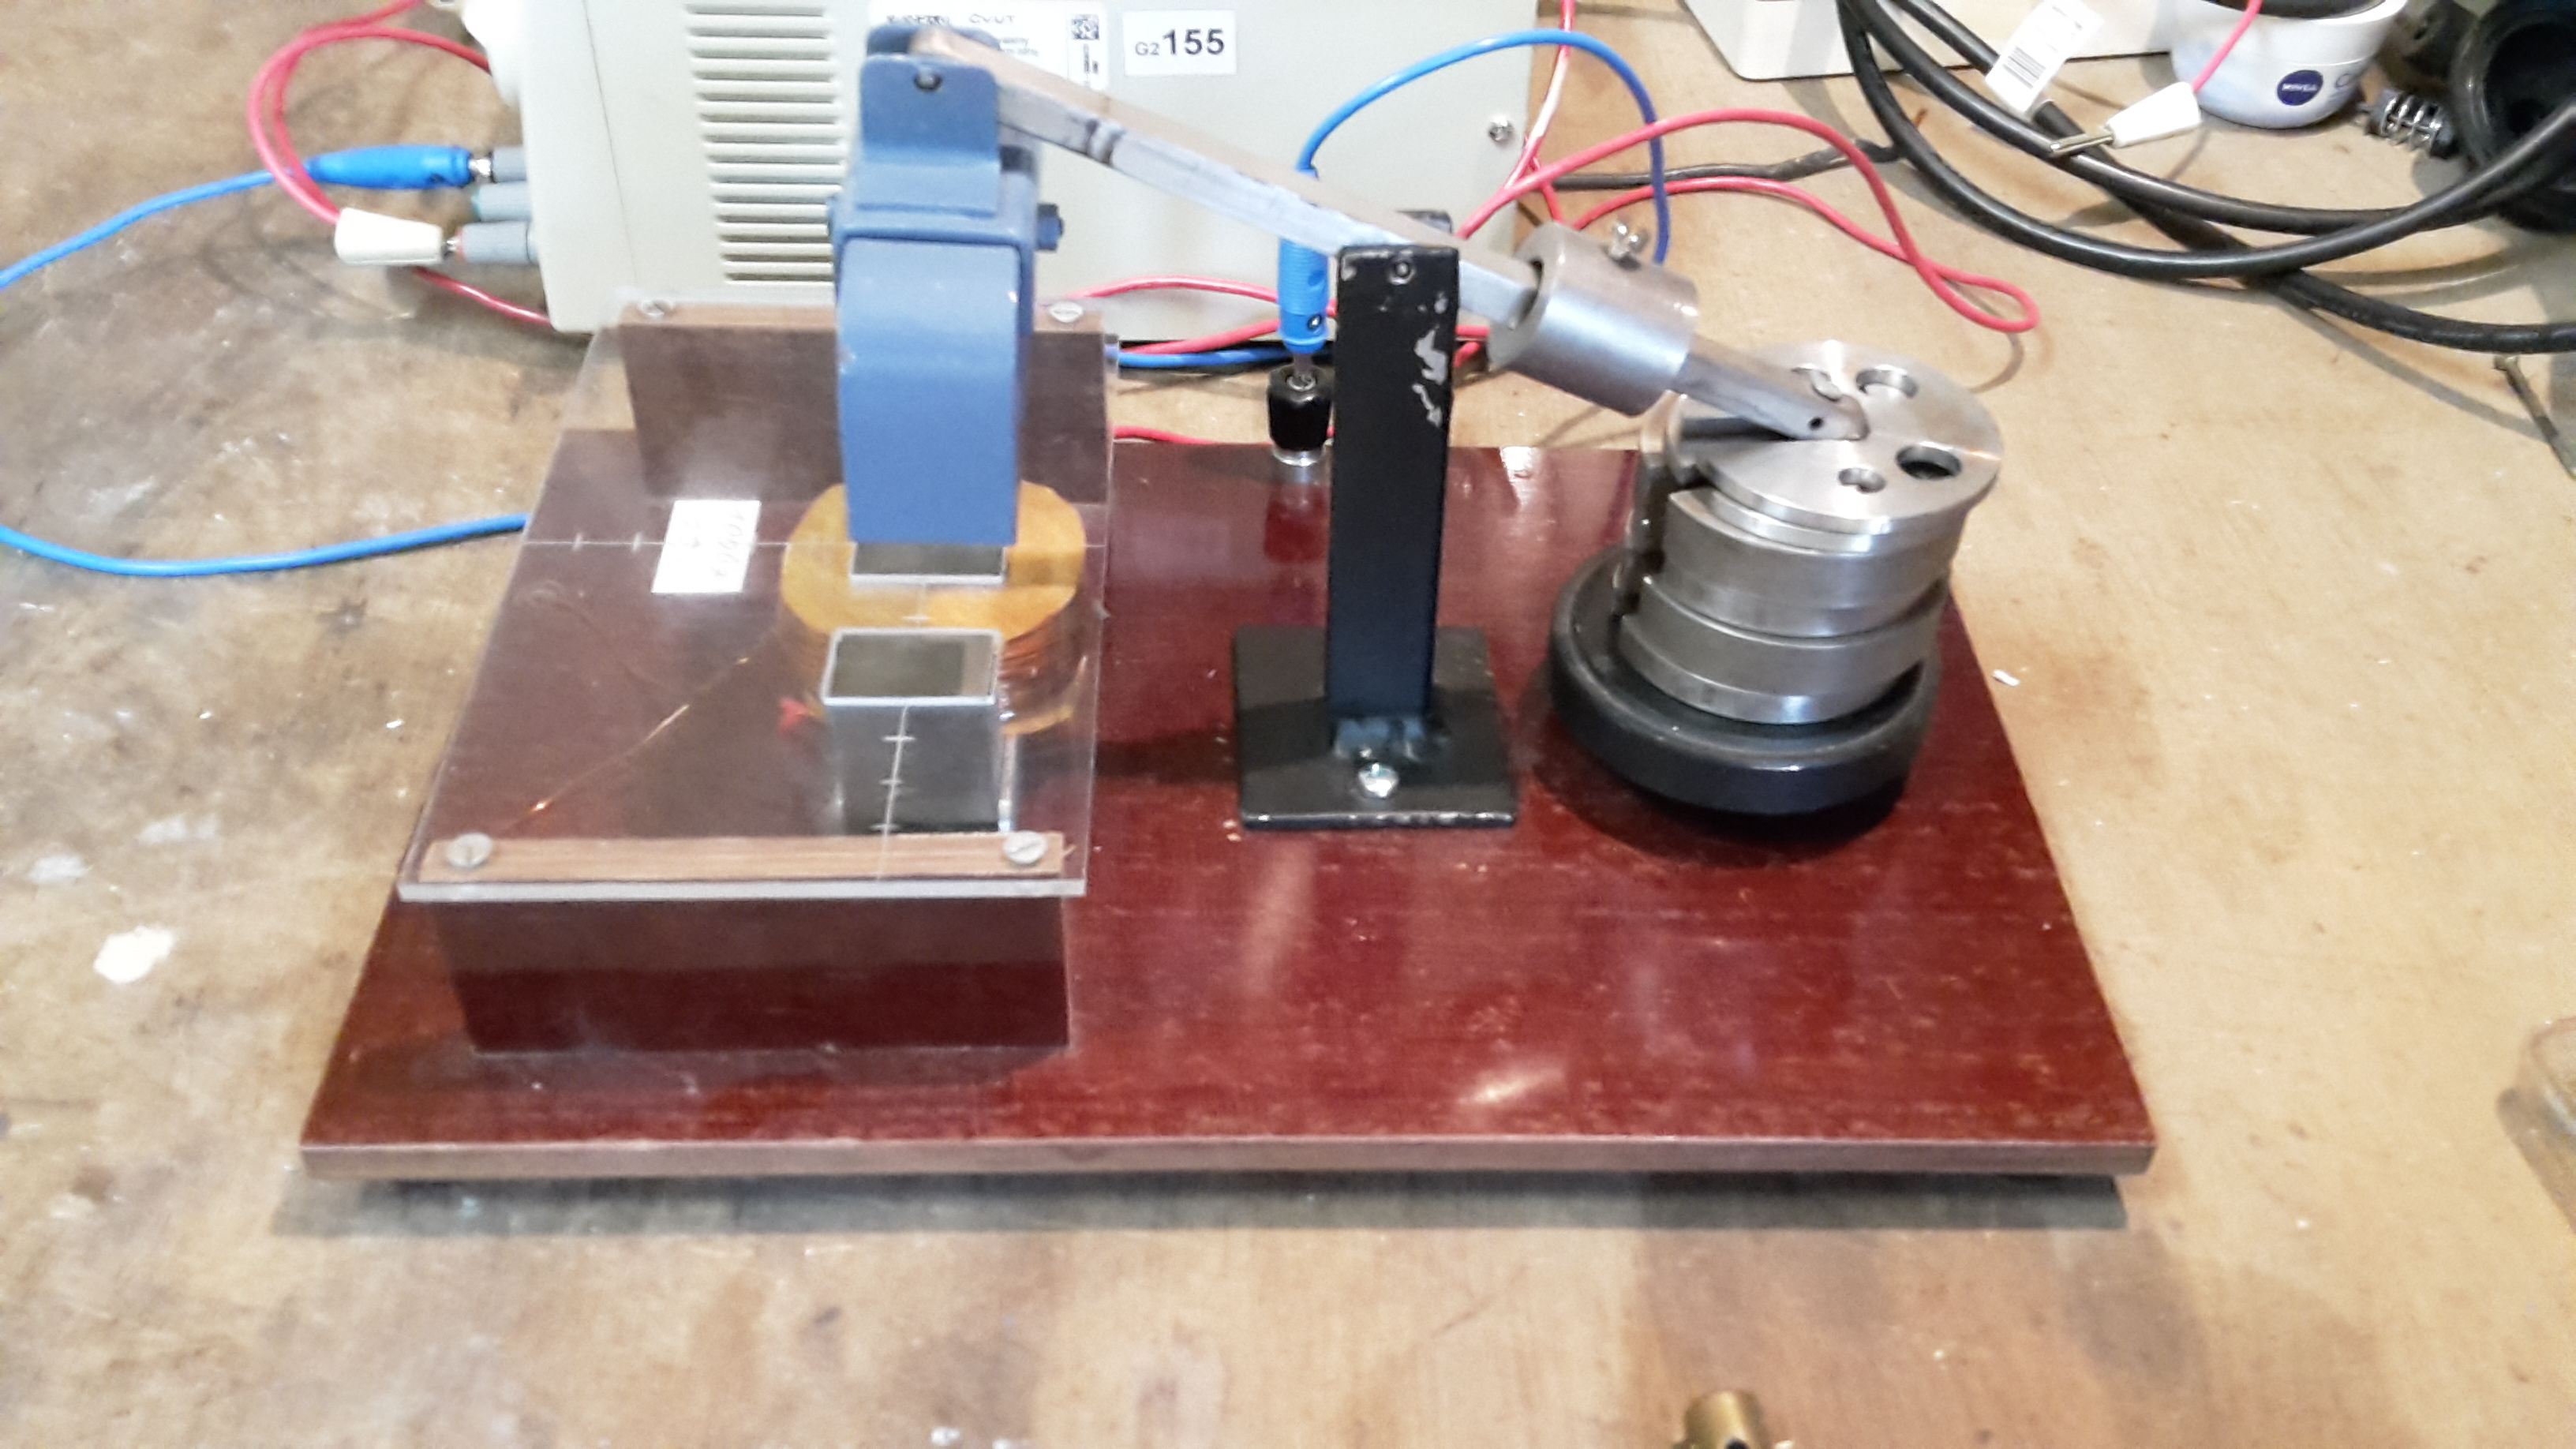
\includegraphics[width=0.5\textwidth]{obrazky/Magnet_2}
   \caption{Obrázek experimentu}
   \label{fig:zadani}
\end{figure}

\section{Teorie}

Energie akumulovaná v takovém magnetickém obvodu je rovna:
\begin{equation} \label{eq:ene}
   W = \frac{1}{2} L I^2 = \frac{1}{2} N^2 G_{m_{celk}} I^2 = \frac{1}{3}N^2 G_m I^2
\end{equation}

Parciální derivací akumulované energie (rce. \ref{eq:ene}) ve směru lze určit přítažnou sílu magnetu:
\begin{equation}
   F = \frac{\partial W}{\partial y} = \frac{1}{3}N^2 I^2 \frac{\partial G_m}{\partial y}
\end{equation}
Tuto derivaci můžeme provést i numericky.

\end{document}